\chapter*{instalasi}


\section*{\textit{ Instalasi Python 3}}
\begin{enumerate}
		\item Clik apk anaconda lau clik install. Selanjutnya clik next.
		\begin{figure}[h]
			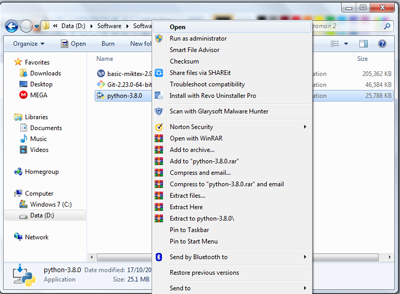
\includegraphics[width=6cm]{figure/1.png}
			\centering
			\caption{install anaconda}
			\end{figure}
		\item Selanjutnya , clik I agree.
			\begin{figure}[h]
			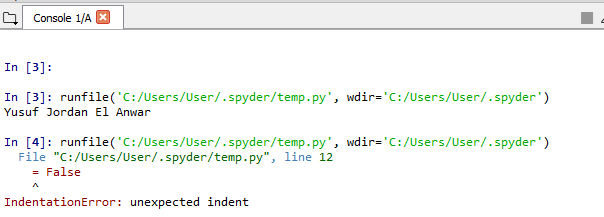
\includegraphics[width=6cm]{figure/2.png}
			\centering
			\caption{licence agreement}
			\end{figure}
		\item Pilih Just me.
			\begin{figure}[h]
			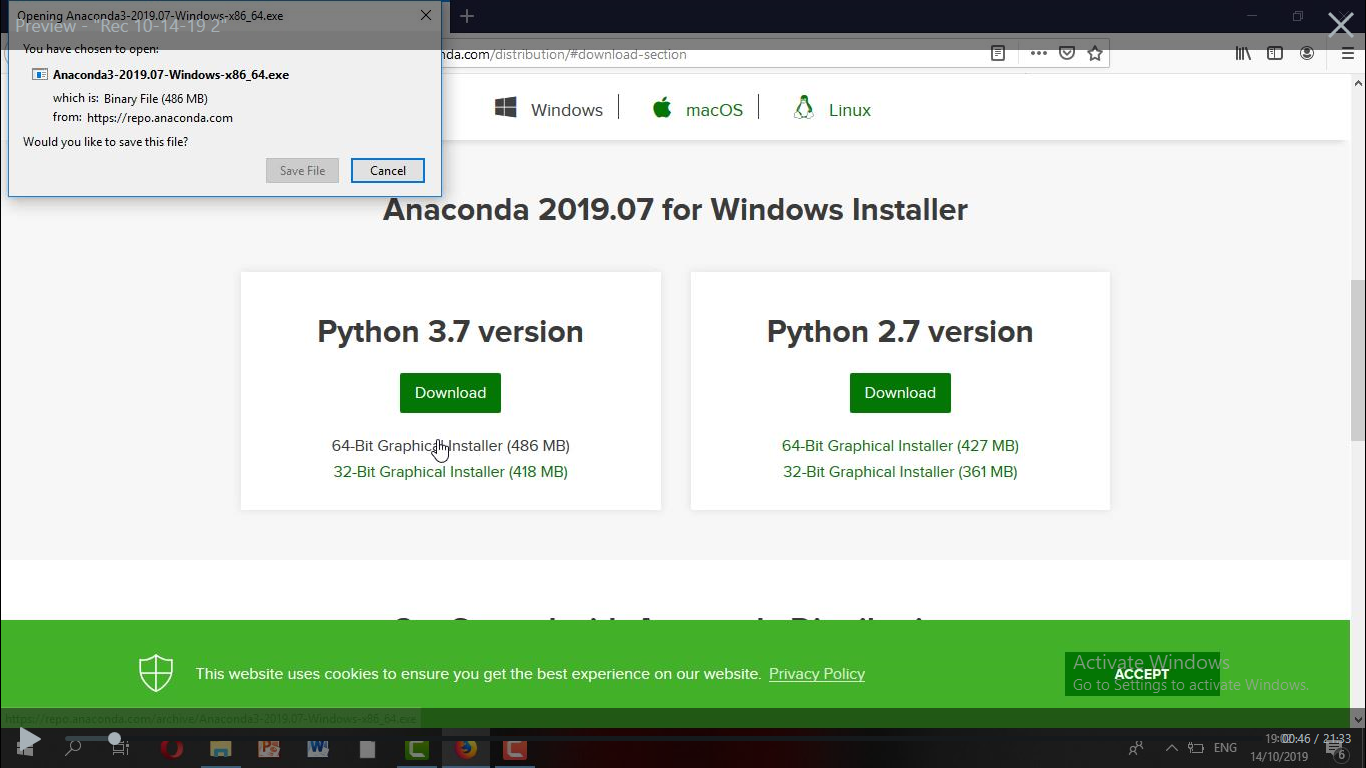
\includegraphics[width=6cm]{figure/3.png}
			\centering
			\caption{installation type}
			\end{figure}
		\item Pilih lokasi penyimpanan yang akan diinstal, lalu clik next.
			\begin{figure}[h]
			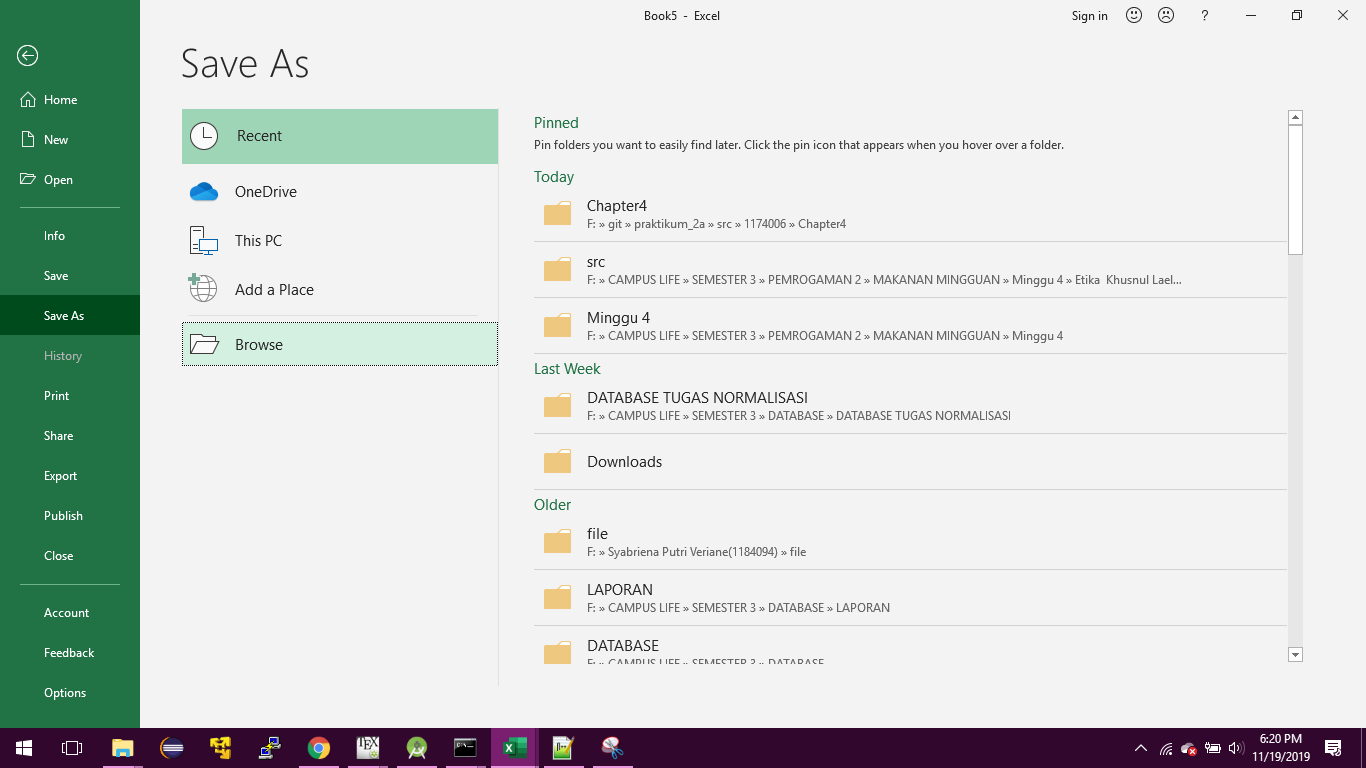
\includegraphics[width=6cm]{figure/4.png}
			\centering
			\caption{lokasi penyimpanan file anaconda}
			\end{figure}
		\item Ceklis bagian ADD Environtment to the Path, hal ini memungkinkan untuk menambahkan environtment anaconda ke dalam path yang ada dalam PC anda. Setelah itu klik next.
			\begin{figure}[h]
			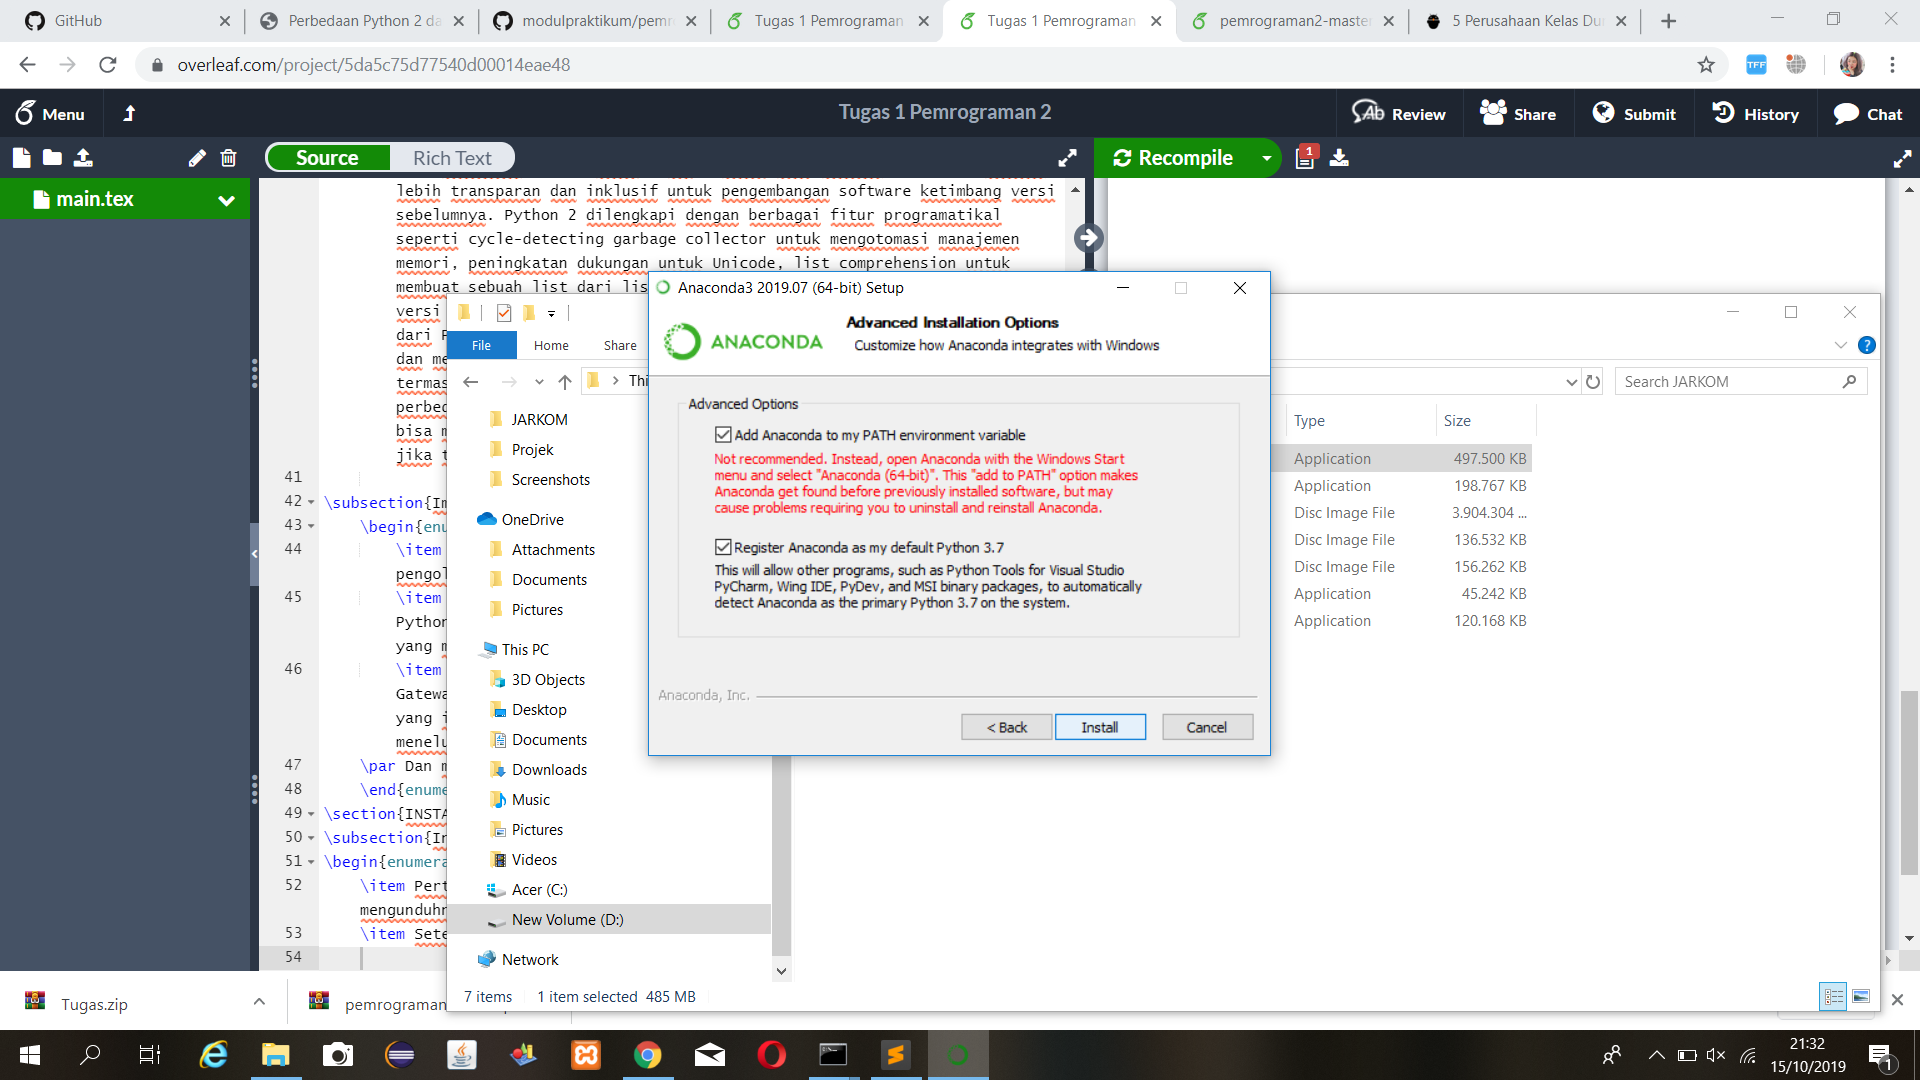
\includegraphics[width=6cm]{figure/5.png}
			\centering
			\caption{menambahkan path environtment}
			\end{figure}
		\item Tunggu instalan sampai selesai.
			\begin{figure}[h]
			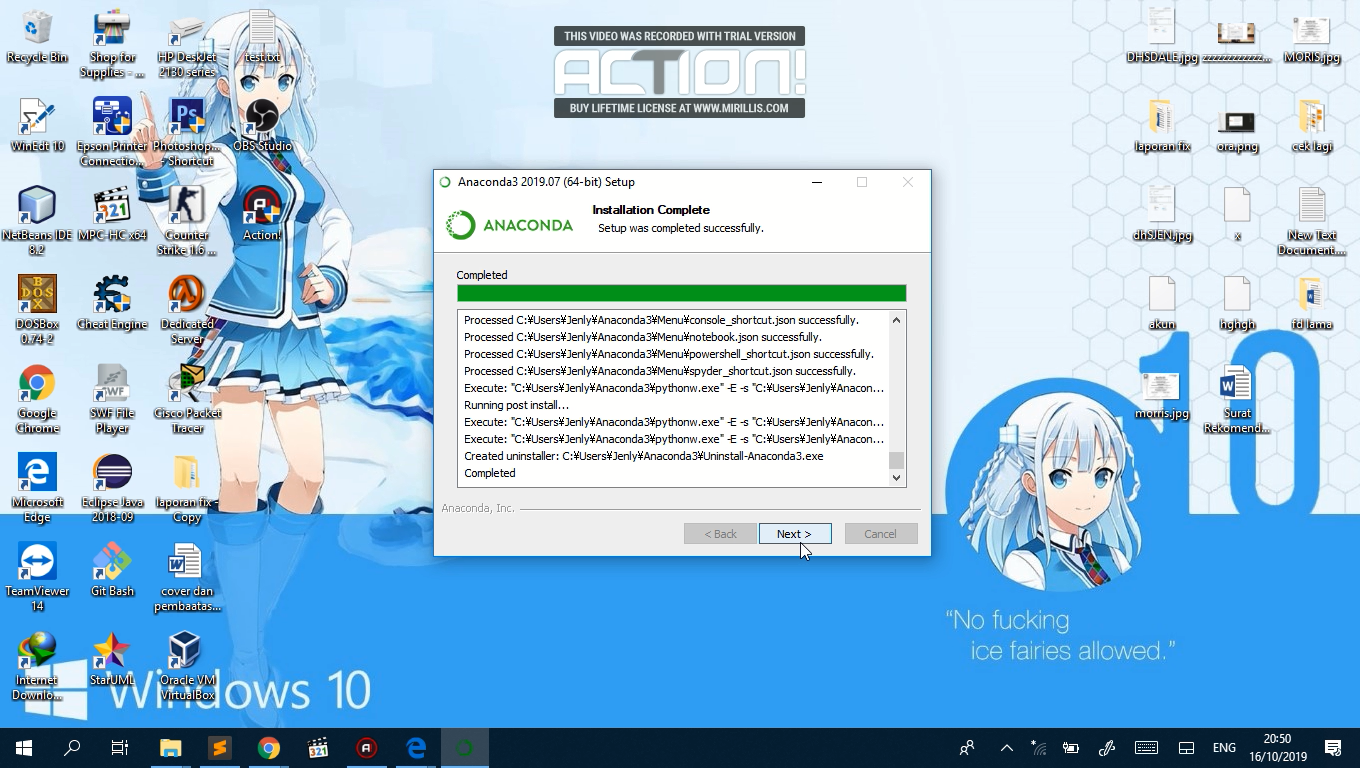
\includegraphics[width=6cm]{figure/7.png}
			\centering
			\caption{proses instalasi}
			\end{figure}
		\item Setelah Instal selesai, lau clik next sampai proses terakhir dan clik finish di akhir proses instal.
			\begin{figure}[h]
			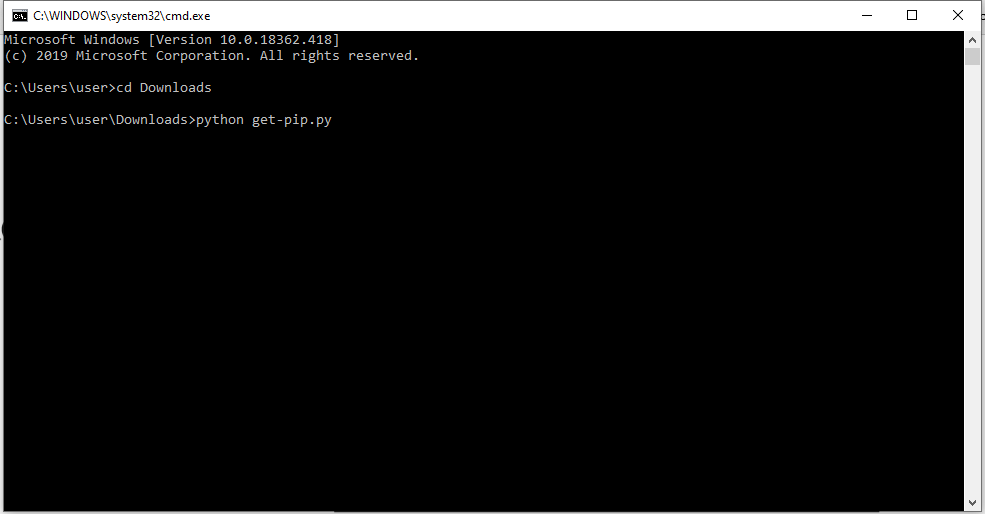
\includegraphics[width=6cm]{figure/8.png}
			\centering
			\caption{instalasi selesai}
			\end{figure}
		\item Click next.	
			\begin{figure}[h]
			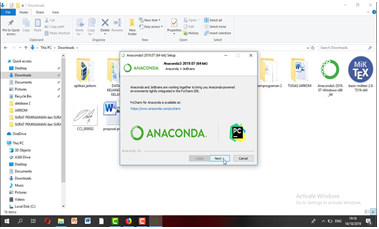
\includegraphics[width=6cm]{figure/9.png}
			\centering
			\caption{instalasi selesai 2}
			\end{figure}
		\item Click next lagi.	
			\begin{figure}[h]
			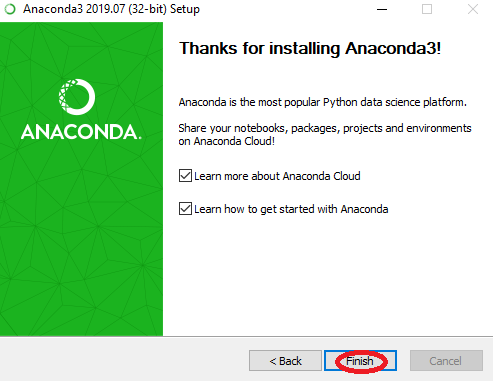
\includegraphics[width=6cm]{figure/10.png}
			\centering
			\caption{instalasi selesai 3}
			\end{figure}
		\item Lalu click finish.	
	\end{enumerate}

\section*{\textit{ Instalasi Pip }}
\begin{enumerate}
		\item Buka Cmd (CommandPrompt)
		\begin{figure}[h]
			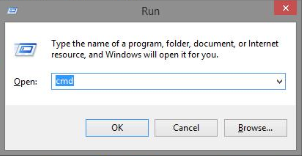
\includegraphics[width=6cm]{figure/pip 1.png}
			\centering
			\caption{klik windows+R, ketik cmd}
			\end{figure}
		\item masuk kedalam direktori yang ada file pip nya.
			\begin{figure}[h]
			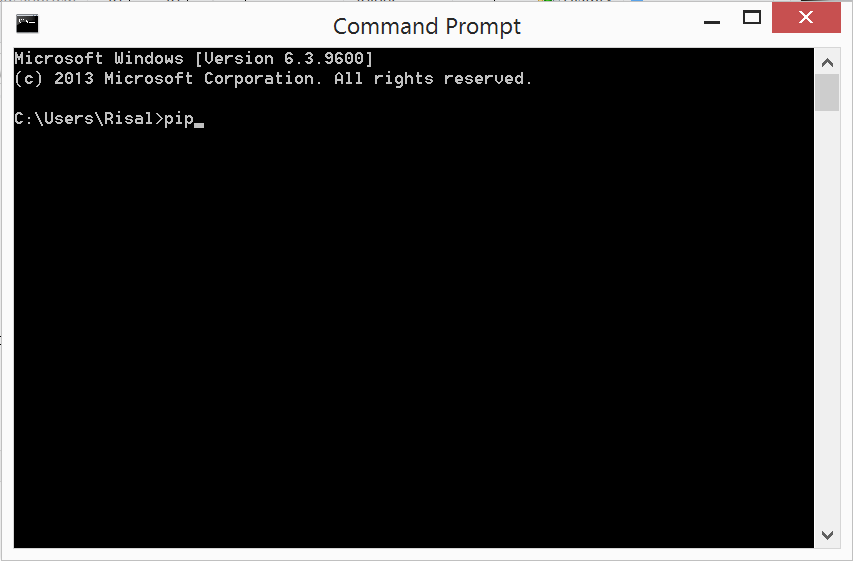
\includegraphics[width=6cm]{figure/pip 2.png}
			\centering
			\caption{ketik pip}
			\end{figure}
		\item Ketikan syntax untuk install pip nya
			\begin{figure}[h]
			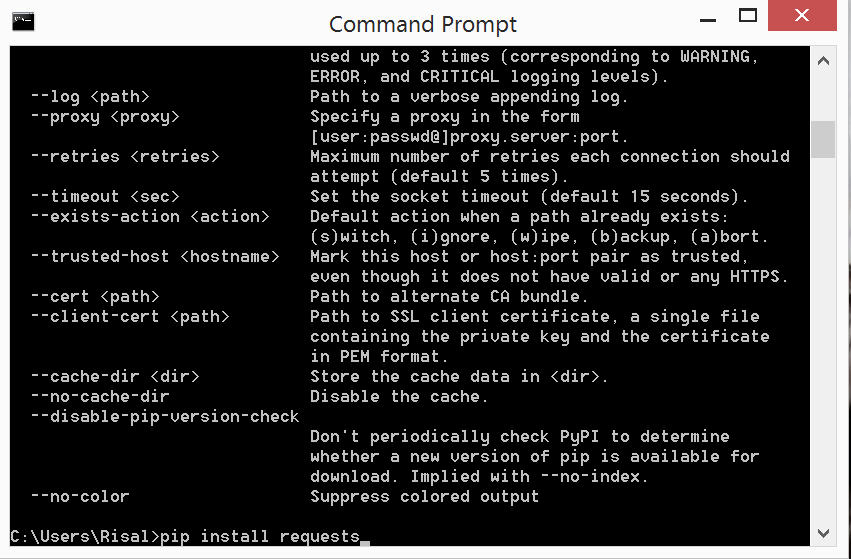
\includegraphics[width=6cm]{figure/pip 3.png}
			\centering
			\caption{ketik pip install requests}
			\end{figure}

		\item Jika sudah ada bacaan successfuly instaled, proses instalasi sudah selesai
			\begin{figure}[h]
			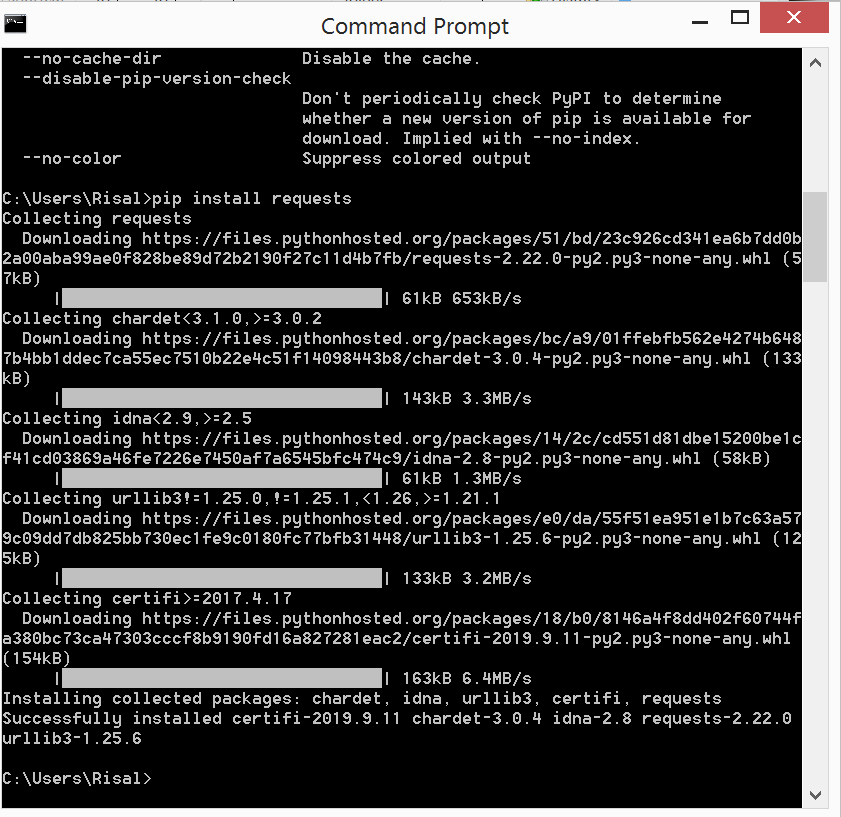
\includegraphics[width=6cm]{figure/pip 4.png}
			\centering
			\caption{Selesai Install}
			\end{figure}
\end{enumerate}

\section*{\textit{ Cara setting environment }}
\begin{enumerate}

\item Buka file exploler, lal click kanan di this pc, pilih properties
\begin{figure}[h]
\centering
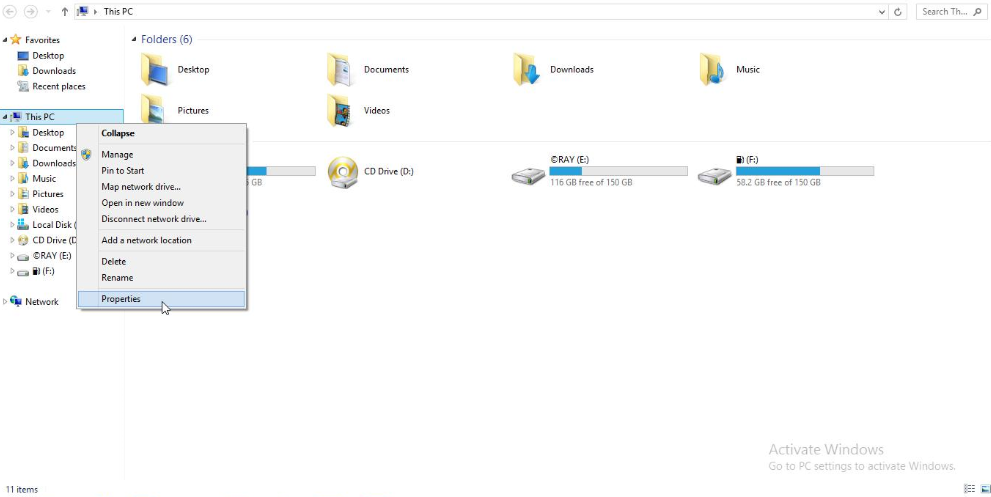
\includegraphics[scale=0.8]{figure/setting1.png}
\caption{membuka file exploler}
\end{figure}

\item Buka advance system settings
\begin{figure}[hb]
\centering
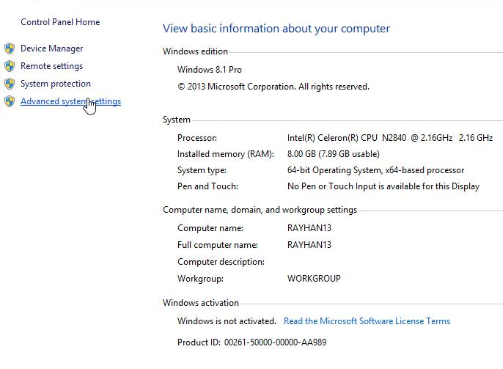
\includegraphics[scale=0.8]{figure/setting2.png}
\caption{membuka advance system}
\end{figure}

\item Click environment variables
\begin{figure}[hb]
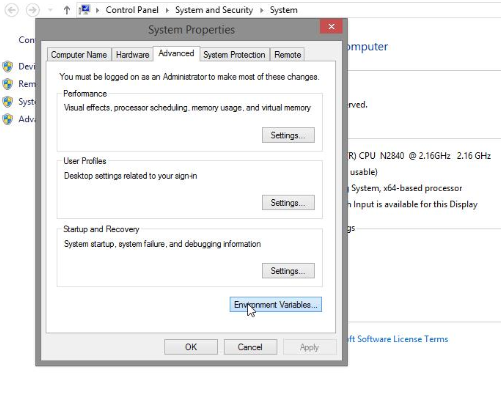
\includegraphics[width=6cm]{figure/setting3.png}
\centering
\caption{membuka environtment variables}
\end{figure}

\item Jika ingin mensetting pilih editt
\begin{figure}[h]
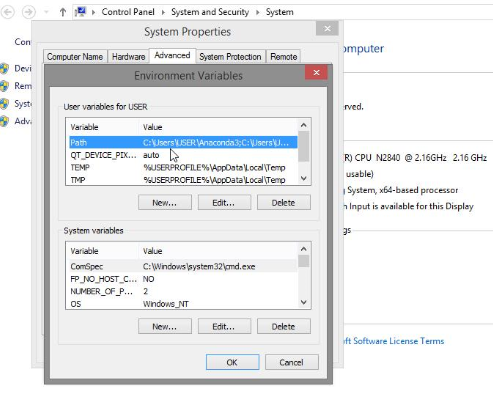
\includegraphics[width=6cm]{figure/setting4.png}
\centering
\caption{mensetting}
\end{figure}
\end{enumerate}
\section*{\textit{ Cara entrepreter melalui cmd window }}
\begin{enumerate}

\item Buka Cmd (CommandPrompt)
		\begin{figure}[h]
			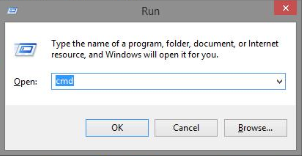
\includegraphics[width=6cm]{figure/entrepeter.png}
			\centering
			\caption{klik windows+R, ketik cmd}
			\end{figure}

\item masuk kedalam direktori yang ada file python nya.
			\begin{figure}[h]
			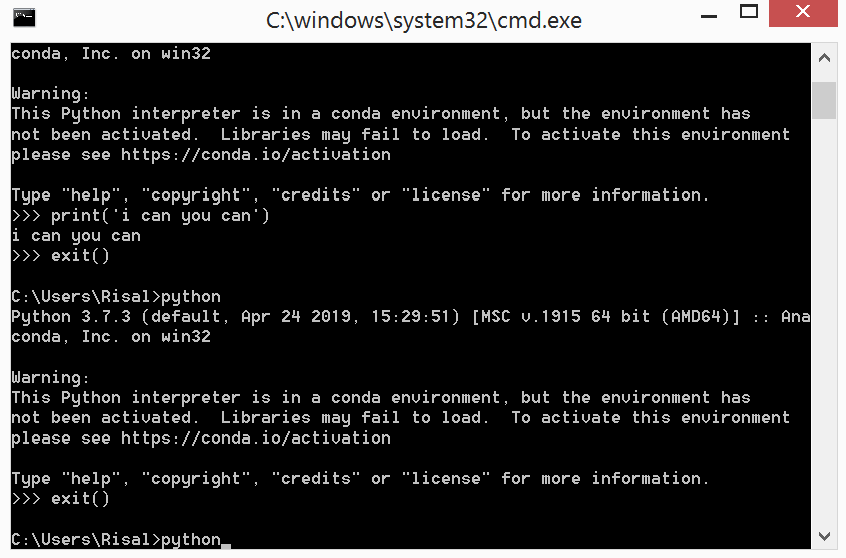
\includegraphics[width=6cm]{figure/entrepreter1.png}
			\centering
			\caption{ketik python}
			\end{figure}
		\item Ketikan syntax entrepreter nya
			\begin{figure}[h]
			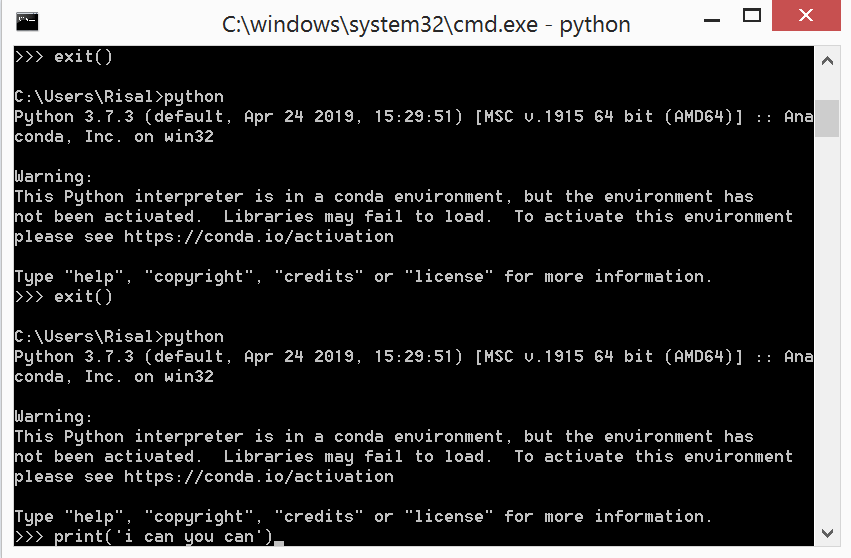
\includegraphics[width=6cm]{figure/entrepreter2.png}
			\centering
			\caption{ketik print('...')}
			\end{figure}

		\item Jika jika benar tulisan yang kita perintahkan akan keluar
			\begin{figure}[h]
			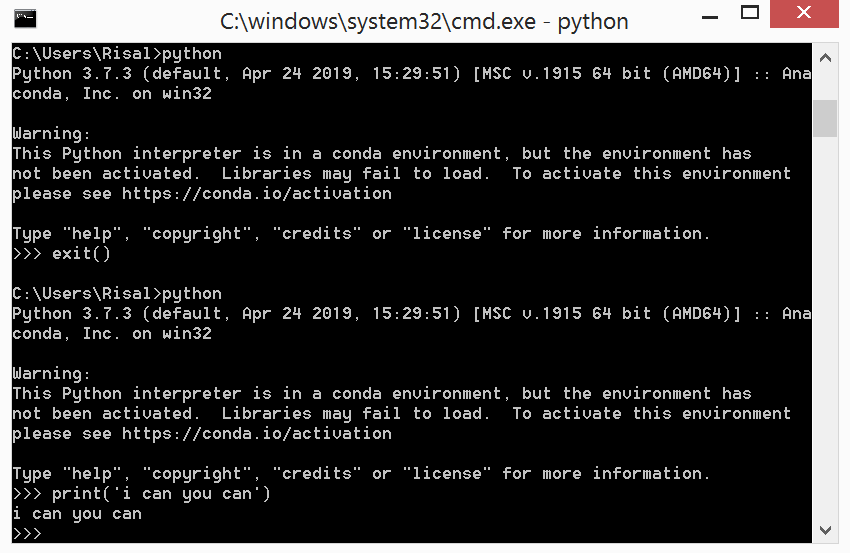
\includegraphics[width=6cm]{figure/entrepreter3.png}
			\centering
			\caption{Selesai}
			\end{figure}


\end{enumerate}

\section*{\textit{ Cara mencetak 'Hello word' di Spyder}}
\begin{enumerate}

\item Buka Anaconda navigator
		\begin{figure}[h]
			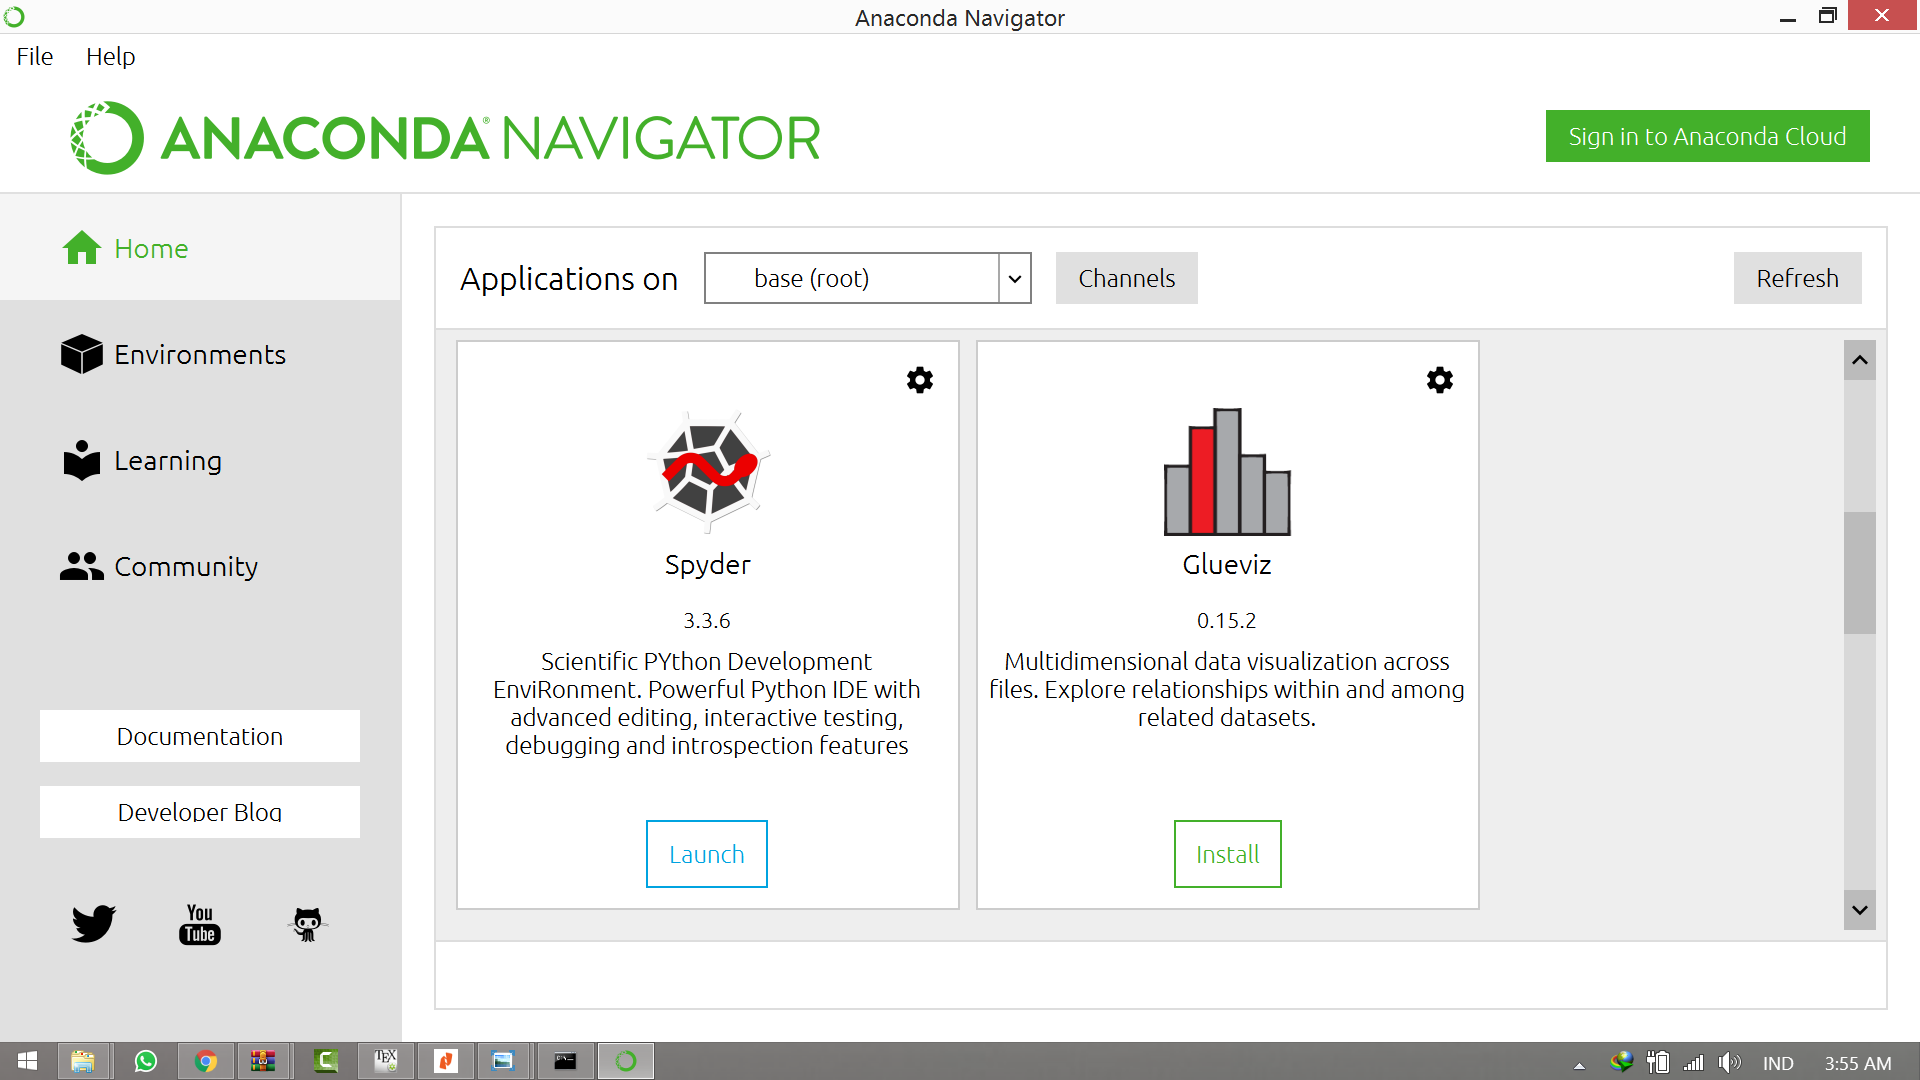
\includegraphics[width=6cm]{figure/anaconda.png}
			\centering
			\caption{buka anaconda navigator lalu klik launch spyder}
			\end{figure}

\item mencetak kalimat 'hello word'.
			\begin{figure}[h]
			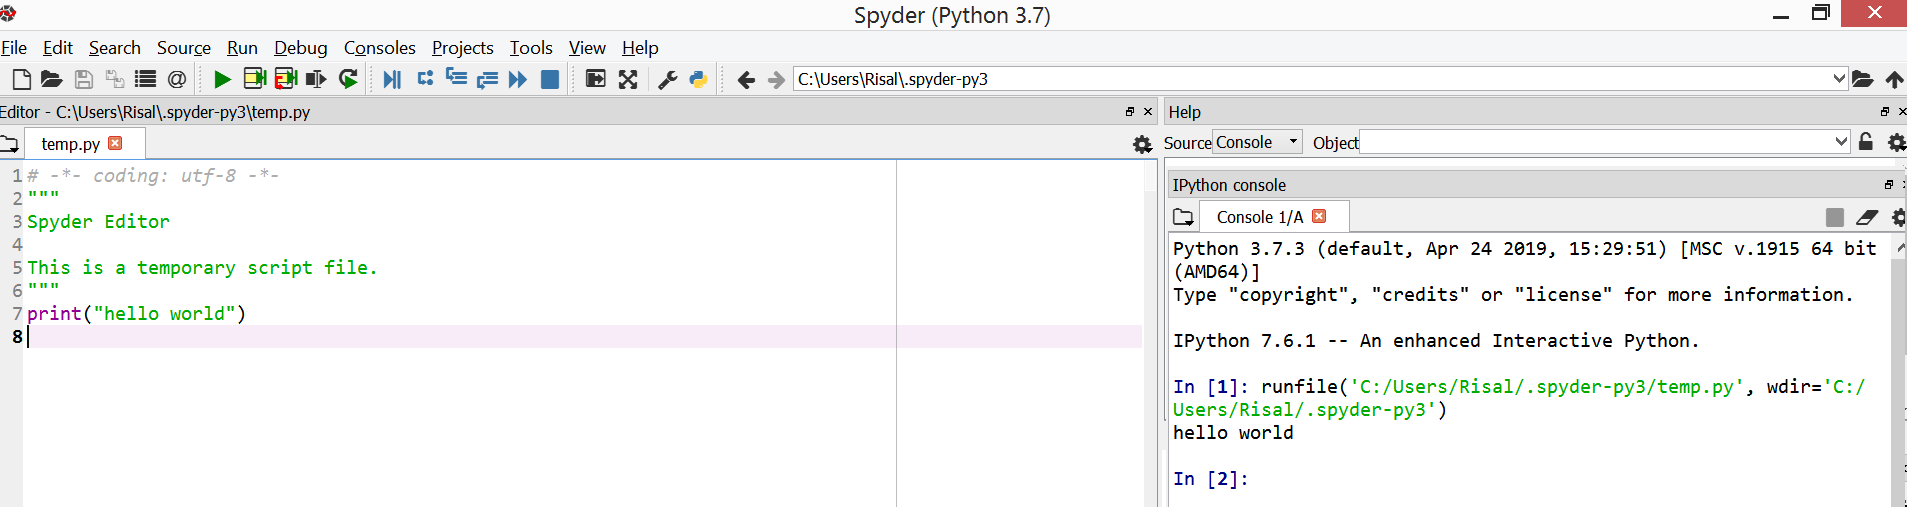
\includegraphics[scale=0.8]{figure/spyder.png}
			\centering
			\caption{ketik print("hello word")}
			\end{figure}
\end{enumerate}

\section*{\textit{Cara Menjalankan Script Auto Login di SIAP}}
\begin{enumerate}
\item ikuti script auto login
		\begin{figure}[h]
			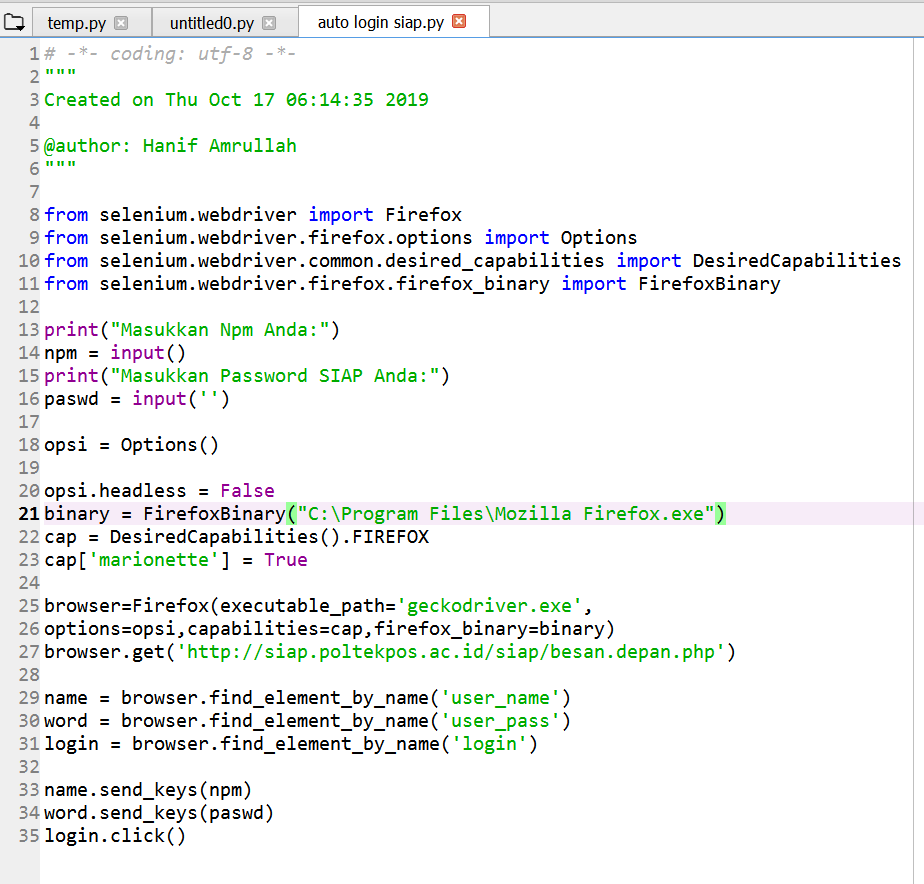
\includegraphics[width=14cm]{figure/siap1.png}
			\centering
			\caption{ketik scriptnya lalu di RUN}
			\end{figure}
\item hasilnya
		\begin{figure}[h]
			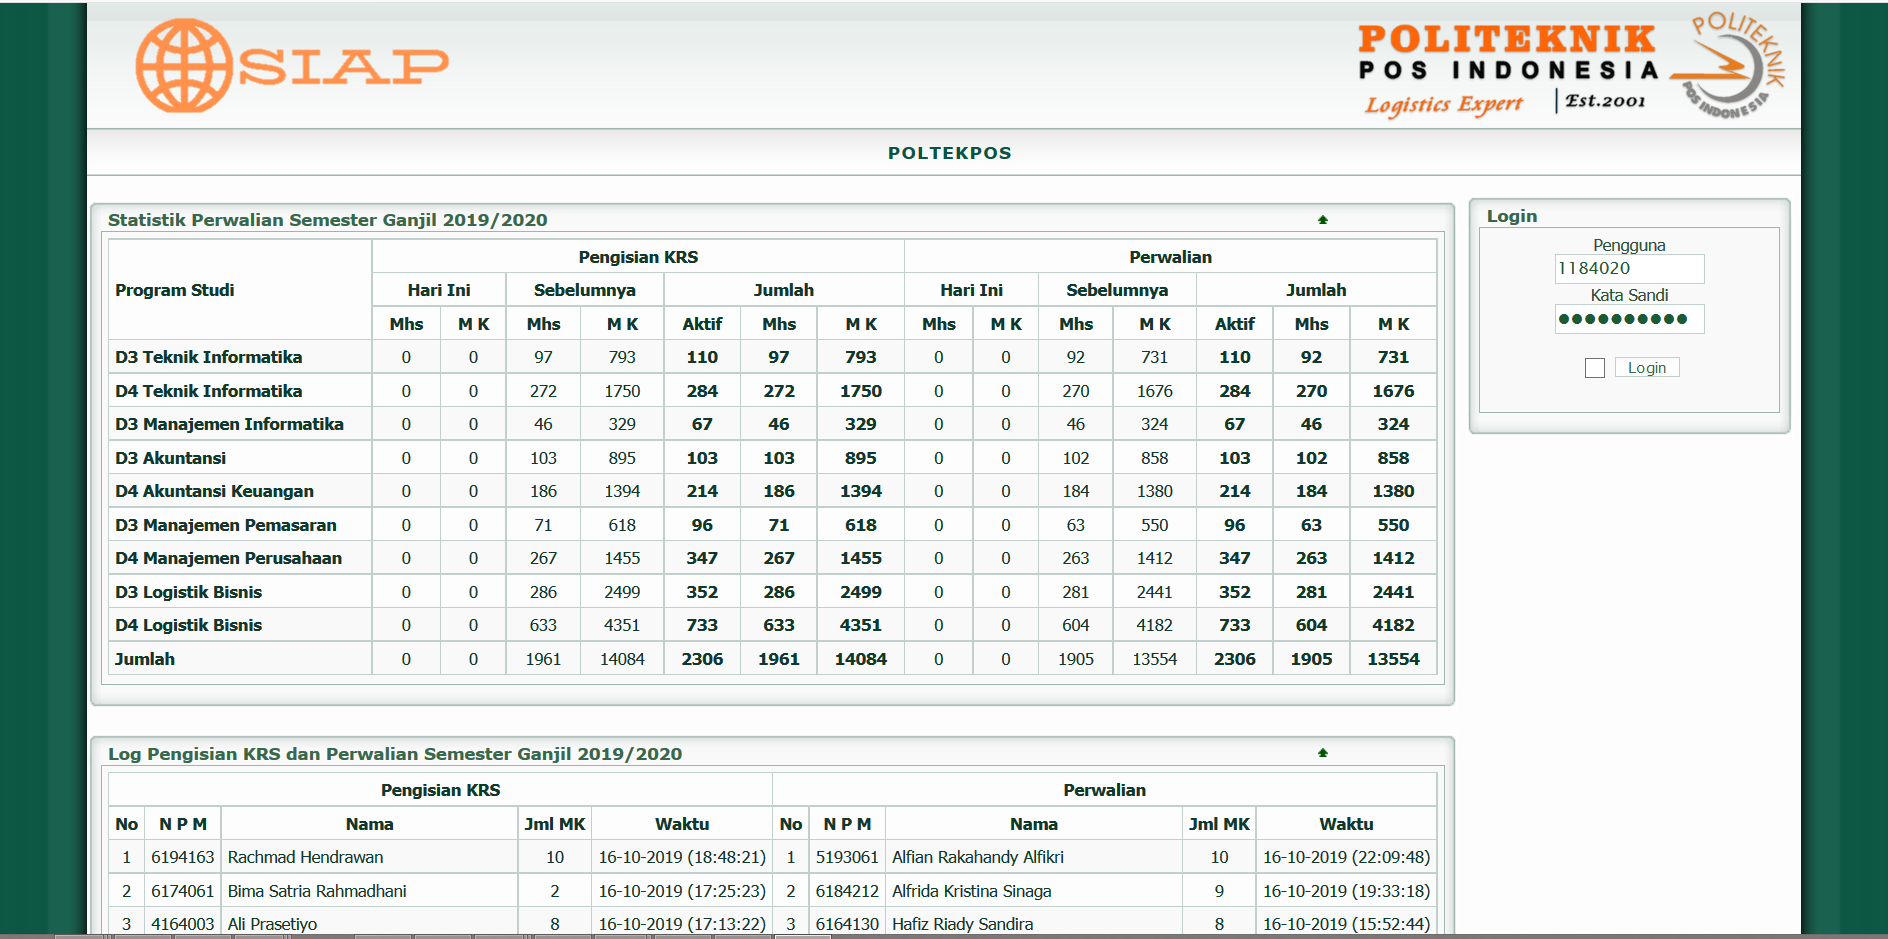
\includegraphics[scale=0.55]{figure/siap2.png}
			\centering
			\caption{tampilannya}
			\end{figure}
\end{enumerate}

\section*{\textit{Cara Pemakaian Variable Explorer}}
\begin{enumerate}
\item Variable Explorer terisi otomatis ketika kita membuat variable
		\begin{figure}[h]
			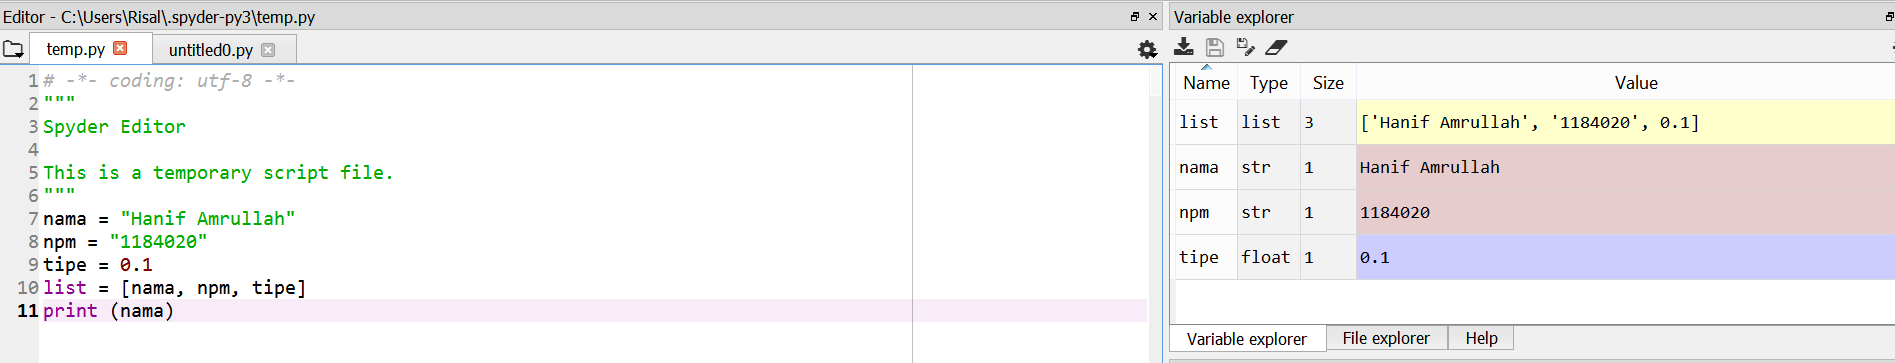
\includegraphics[width=10cm]{figure/variabel.png}
			\centering
			\caption{ketik scriptnya lalu di RUN}
			\end{figure}
\end{enumerate}

\section*{\textit{pejelasan Indentasi}}
\begin{verbatim}
Indentasi merupakan salah satu cara untuk merapikan sintaks pemrograman yang hendak ditulis yang selalu berhubungan dengan kurung kurawal ‘{}’ dalam memulai dan mengakhiri suatu scope pemrograman dan compiler, seperti salah satunya bahasa pemrograman python. error indentasi dapat terjadi apabila syntax tidak menggunakan space. Contoh yang benar (menggunakan tab/spasi sebagai indentasi):

# percabangan if
if username == 'hanif':
	print("Selamat Datang brother")
	print("jangan Lupa Solat")
	
# blok percabangan for
for i in range(10):
 print i
 

contoh yang salah (tidak menggunakan tab/spasi):

if username == 'hanif':
print("Selamat Datang brother")
print("jangan Lupa Solat")
	
# blok percabangan for
for i in range(10):
print i
\end{verbatim}

\section*{\textit{Jenis-Jenis Error Indentasi}}
\begin{enumerate}
\item indentitaionError : unexpected indent. Error terjadi apabila syntax kekurangan tab atau spasi
		\begin{figure}[h]
			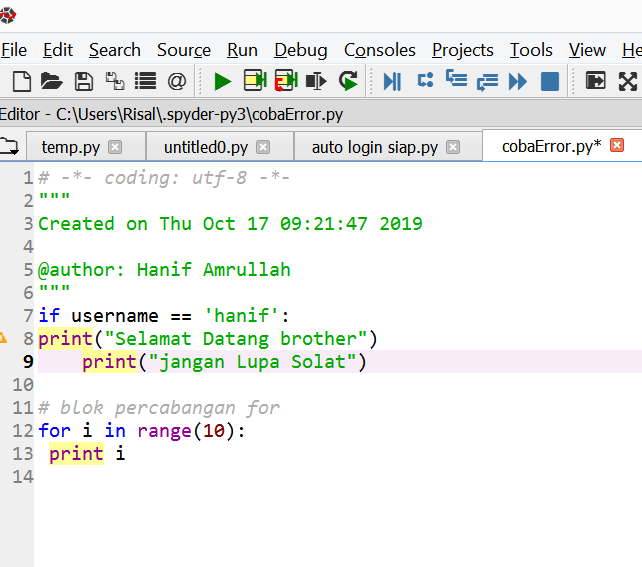
\includegraphics[width=10cm]{figure/Error1.png}
			\centering
			\caption{Indentasi}
			\end{figure}
\item Apabila di running akan muncul error sepeti berikut :
		\begin{figure}[h]
			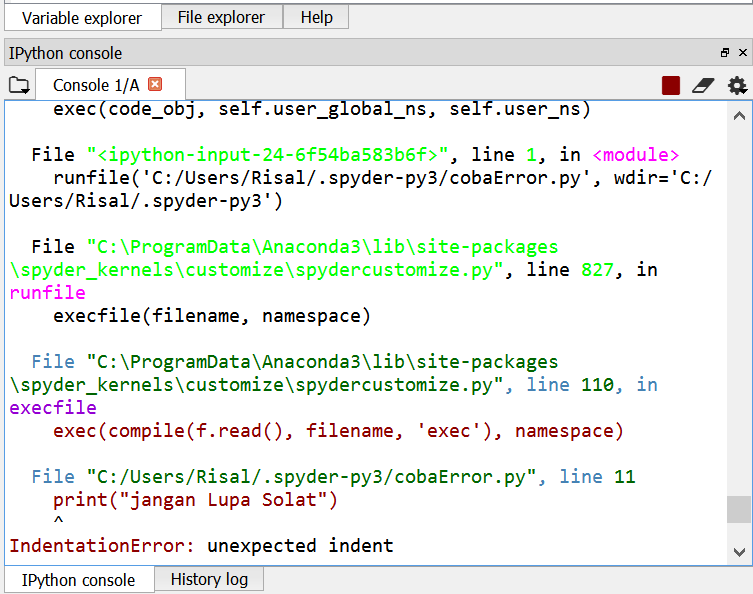
\includegraphics[width=10cm]{figure/Error2.png}
			\centering
			\caption{Error Indentasi}
			\end{figure}
\end{enumerate}
\section*{\textit{Cara Membaca Error}}
\begin{enumerate}
\item Cari error di line beberapa error terjadi, contohnya pada gambar pada line 11
		\begin{figure}[h]
			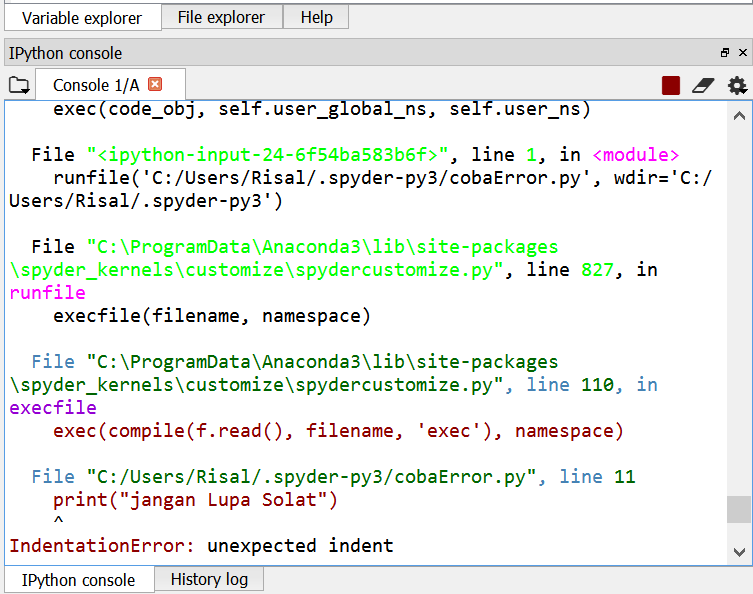
\includegraphics[width=10cm]{figure/Error3.png}
			\centering
			\caption{Error}
			\end{figure}
\end{enumerate}
\section*{\textit{Cara Menangani Error}}
\begin{enumerate}
\item Cara menangani error
		\begin{figure}[h]
			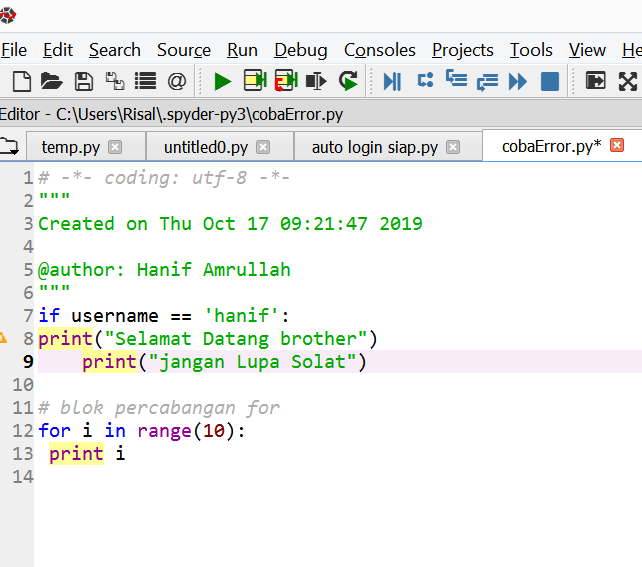
\includegraphics[width=10cm]{figure/Error4.png}
			\centering
			\caption{Syntax Error}
			\end{figure}
\item Berikut syntax yang sudah diperbaiki dengan tab/spasi di indentasi
		\begin{figure}[h]
			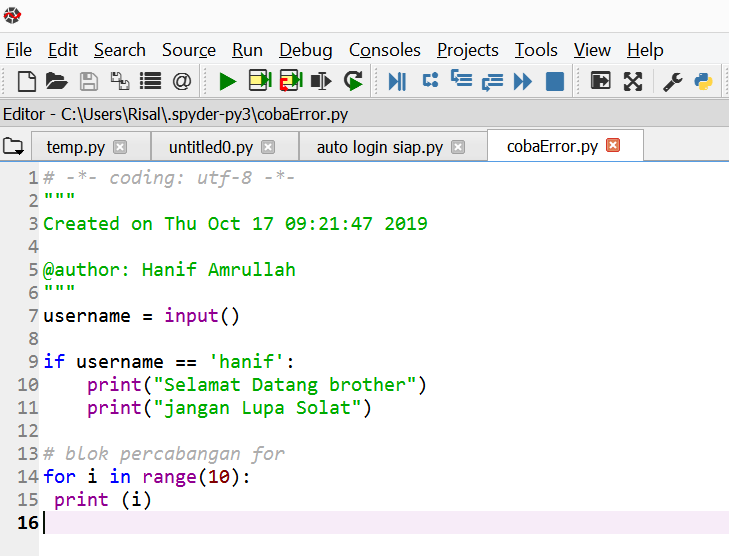
\includegraphics[width=10cm]{figure/Error5.png}
			\centering
			\caption{Syntax yang sudah diperbaiki}
			\end{figure}
\end{enumerate}